%%%%%%%%%%%%%%%%%%%%%%%%%%%%%%%%%%%%%%%%%%%%%%%%%%%%%%%%%%%%%%%%%%%%%%%%%
% Antes de correr el código:
% 1. Ingresar al Menu
% 2. Cambiar la opción "Compiler" a XeLaTeX
% 3. Cambiar la opción "TeX live version" a 2020 (opacidad de la imagen)
%%%%%%%%%%%%%%%%%%%%%%%%%%%%%%%%%%%%%%%%%%%%%%%%%%%%%%%%%%%%%%%%%%%%%%%%%
\documentclass[10pt]{article}
\usepackage[T1]{fontenc}
\usepackage[utf8]{inputenc}
\usepackage[english]{babel}
\usepackage{listings}
\lstset{language=R}
\usepackage[a4paper]{geometry}
\usepackage[dvipsnames]{xcolor}
\usepackage[framemethod=TikZ]{mdframed}
\usepackage{graphicx,tikz}
\usepackage{array}
\usepackage{float}
\usepackage{tocloft}
\setlength{\cftsecnumwidth}{2em}
\usepackage{xspace}
\usepackage{tcolorbox}
\tcbuselibrary{listings}

\newtcblisting{cc}{
  listing only,
  nobeforeafter,
  after={\xspace},
  hbox,
  tcbox raise base,
  fontupper=\ttfamily,
  colback=lightgray,
  colframe=lightgray,
  size=fbox
  }

\geometry{top=2.54cm, bottom=2.54cm, left=2.54cm, right=2.54cm}

\usepackage{url}
\usepackage{lipsum} 
\usepackage{wrapfig}
\usepackage{subcaption}
\usepackage{multicol}

%==========================================
%======     FUENTE PARA CÓDIGOS      ======
%==========================================
\definecolor{codegreen}{rgb}{0,0.6,0}
\definecolor{codegray}{rgb}{0.1,0.1,0.1}
\definecolor{backcolour}{rgb}{0.98,0.98,0.98}

\lstdefinestyle{mystyle}{
  backgroundcolor=\color{backcolour},   
  commentstyle=\color{codegreen},
  keywordstyle=\color{blue},
  numberstyle=\tiny\color{codegray},
  stringstyle=\color{codegreen},
  basicstyle=\ttfamily\footnotesize,
  breakatwhitespace=false,         
  breaklines=true,                 
  captionpos=b,                    
  keepspaces=true,                 
  numbers=left,                    
  numbersep=5pt,                  
  showspaces=false,                
  showstringspaces=false,
  showtabs=false,                  
  tabsize=2
}

%==========================================
%==========     ESTILO TITLE     ==========
%==========================================
\newcommand{\City}[1]{\def\City{#1}}

\makeatletter         
\renewcommand\maketitle{
\begin{flushleft}
{\textcolor{black}{\huge \bfseries \@title }}\\[1ex]
\rule{\textwidth}{0.6pt}\\
\end{flushleft}
\vspace{-0.5cm}

\begin{flushleft}
\textcolor{black}{{\large  \@author} }\\[2ex]
\end{flushleft} } % Note the extra }
\makeatother

%==========================================
%==========    ESTILO CAPTION    ==========
%==========================================
\usepackage{caption}
\captionsetup[table]{name=Tabla ,textfont={it}, labelfont={bf},
                     justification=centering,
                     width =\dimexpr \textwidth-0.5cm\relax}
\captionsetup[figure]{textfont={it}, labelfont={bf},
                      justification=centering, skip=2pt,
                      belowskip=-5pt}
                      
%==========================================
%==========     ESTILO ITEM      ==========
%==========================================
\renewcommand{\labelitemi}{$\bullet$} 
\renewcommand{\labelitemii}{$\circ$} 
\renewcommand{\labelitemiii}{$\cdot$} 

%==========================================
%===    LINKS (Agregar Hyperlinks)     ====
%==========================================
\usepackage[style=apa,
            urldate=long]{biblatex} 
\addbibresource{Bib.bib}

\DeclareSourcemap{
  \maps[datatype=bibtex]{
    \map{
      \step[fieldsource=note, final]
      \step[fieldset=addendum, origfieldval, final]
      \step[fieldset=note, null]}
      }
}

\DefineBibliographyStrings{english}{urlseen = {Accessed }    
}

\usepackage[colorlinks=true,linkcolor=RoyalBlue,
            citecolor=RoyalBlue,urlcolor=RoyalBlue]{hyperref}

%==============================================================
%==============================================================
\title{ }

%%%%%%%%%%%%%%%%%%%%%%%%%%%%%%%%%%%%%%%%%%%%%%%%%%%%%%%%%%%%%%%
%%%%%%%%%%%%                 INICIO                %%%%%%%%%%%% 
%%%%%%%%%%%%%%%%%%%%%%%%%%%%%%%%%%%%%%%%%%%%%%%%%%%%%%%%%%%%%%%
\begin{document}

\begingroup
\let\clearpage\relax % prevent extra page breaks
\thispagestyle{empty}
\begin{center}
{\huge \bfseries Universidad de los Andes}

\vspace{25pt}
{\LARGE \bfseries Departamento de Ingeniería de Sistemas}

\vspace{15pt}

\includegraphics[width=100pt]{images/logo.png} 

\vspace{35pt}
{\LARGE \bfseries Laboratorio \#2: Análisis De Protocolos De La Capa De Aplicación}
\vspace{55pt}

{\Large \bfseries ISIS3204 - Infraestructura de Comunicaciones}


\vspace{100pt}
{\Large \bfseries Grupo 3: }

\end{center}

\begin{flushleft}
  \setlength{\parskip}{0pt}
  \setlength{\itemsep}{0pt}
  \hspace*{4cm}\large\bfseries Juan Esteban Quiroga - 202013216

  \hspace*{4cm}\large\bfseries Juan Manuel Rodriguez - 202013372

  \hspace*{4cm}\large\bfseries Andres Felipe Ortiz - 201727662
\end{flushleft}

\begin{center}
\vspace{60pt}

\Large\bfseries 2025-10
\end{center}

\mbox{}
\endgroup

\clearpage

\tableofcontents
\clearpage


\renewcommand{\thesection}{\arabic{section}}
\section*{Introducción}
\addcontentsline{toc}{section}{Introducción}
En este laboratorio configuramos y probamos algunos servicios de red: DNS, HTTP/HTTPS, FTP, VoIP y RTMP, usando una topología a pequeña escala. Con Wireshark analizamos la conectividad de estos servicios en dicha red. Este laboratorio nos ayudó a entender la interacción de protocolos importantes que soportan la comunicación en redes de computadores. En la figura 1 mostramos las IPs estáticas que usamos para este laboratorio. (Es importante que estas IPs no sean dinamicas por DHCP ya que esto asegura direccionamiento constante y facilidad de configuración stable en la red.) La asignación de direcciones inició en $172.20.10.5$ porque el gateway de la red es el hotspot del iPhone en $172.20.10.1$, dejando libres las direcciones previas para posibles equipos de infraestructura y evitando conflictos.


\begin{figure}[H]
    \centering
    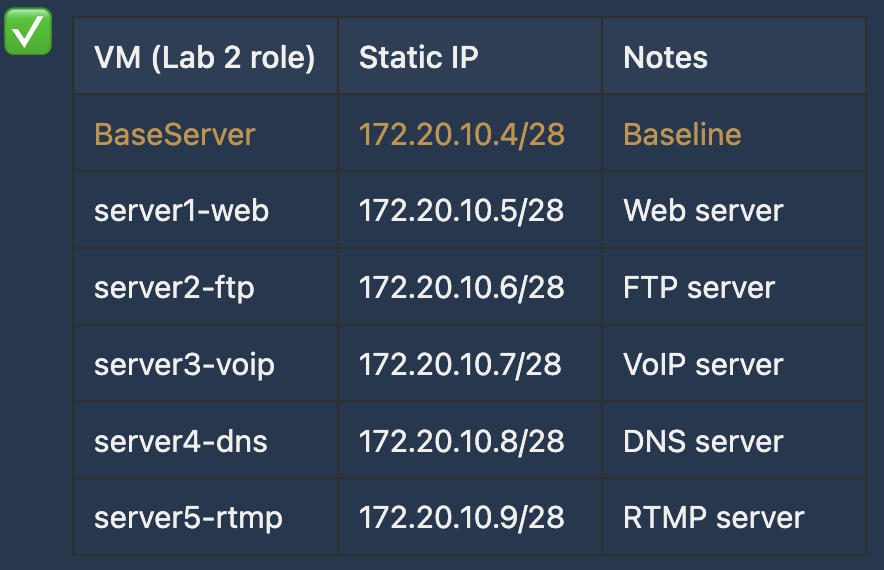
\includegraphics[width=0.55\textwidth]{lab-02-screenshots/server-ips.png}
    \caption{Configuración de IPs estáticas}
\end{figure}


%==============================================================
%=====================   8.1   ================================
%==============================================================
\renewcommand{\thesection}{8.\arabic{section}}
\setcounter{section}{0}
\section{Prueba ping}

En esta sección se verifica la conexión básica entre el cliente y los servidores DNS y FTP mediante pings con el protocolo ICMP, asegurando la conectividad antes de analizar los demás protocolos.

\subsection{Prueba de conectividad al servidor DNS}

Desde el cliente se enviaron pings (echo requests ICMP ) al servidor DNS utilizando su dirección IP (\textbf{172.20.10.8}). El tráfico generado se capturó y se guardó en el archivo \textcolor{blue}{\texttt{Ping\_DNS\_IP.pcap}}. El archivo fue abierto en Wireshark y se aplicó el filtro icmp para observar únicamente los paquetes de ping. Se registraron la dirección IP de origen, dirección IP de destino, dirección MAC de origen y dirección MAC de destino en las tramas capturadas.

\begin{figure}[H]
    \centering
    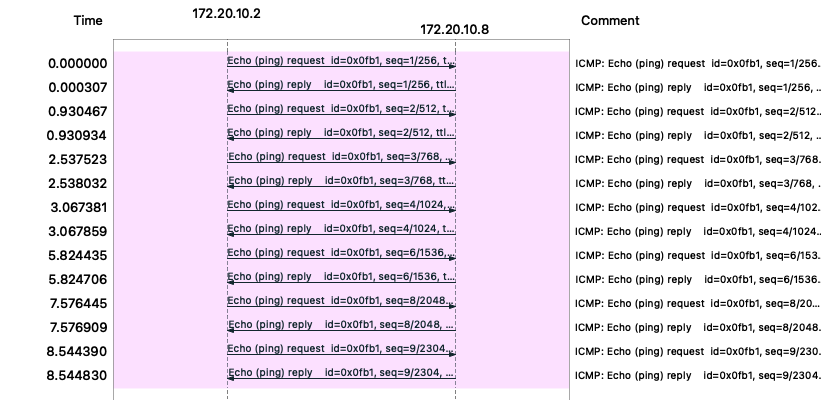
\includegraphics[width=0.85\textwidth]{lab-02-screenshots/8.1-DNS-flow}
    \caption{Flujo de packets en DNS ping}
\end{figure}


\begin{figure}[H]
    \centering
    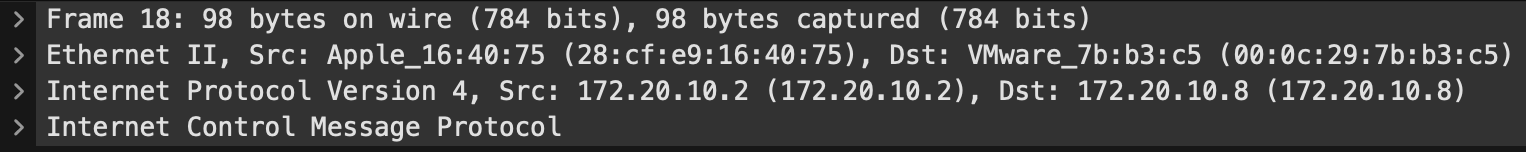
\includegraphics[width=0.85\textwidth]{lab-02-screenshots/8.1-DNS-data}
    \caption{Evidencia de IPs y MACs origen/destino}
\end{figure}

\begin{figure}[H]
    \centering
    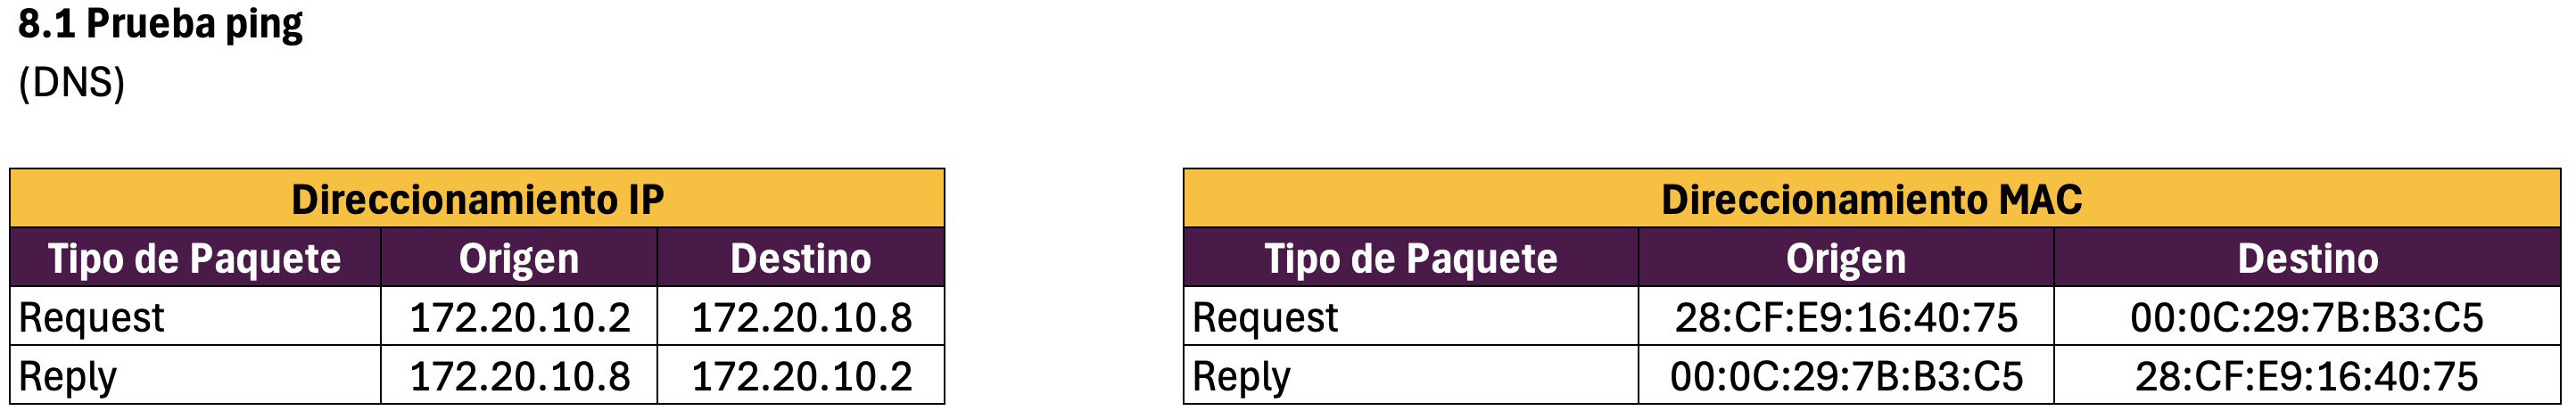
\includegraphics[width=0.85\textwidth]{lab-02-screenshots/8.1-DNS-ping-table}
    \caption{Tabla de IPs y MACs origen/destino}
\end{figure}


\subsection{Prueba de conectividad al servidor FTP}

Desde el cliente se enviaron pings al servidor FTP utilizando su dirección IP. El tráfico generado se capturó y se guardó en el archivo \textcolor{blue}{\texttt{Ping\_FTP\_IP.pcap}} El archivo fue analizado en Wireshark con el filtro icmp. Se identificaron las direcciones IP y MAC correspondientes a los paquetes de solicitud y respuesta.

\begin{figure}[H]
    \centering
    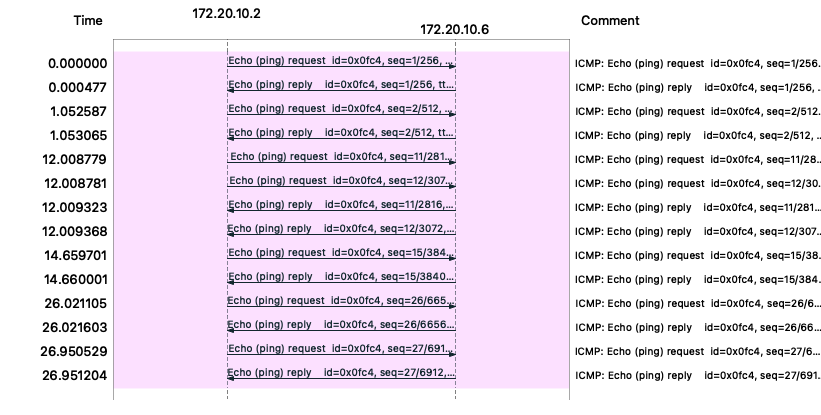
\includegraphics[width=0.85\textwidth]{lab-02-screenshots/8.1-FTP-flow}
    \caption{Flujo de packets en FTP ping}
\end{figure}


\begin{figure}[H]
    \centering
    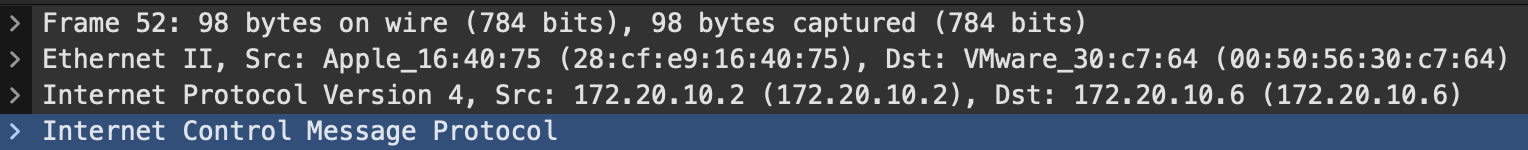
\includegraphics[width=0.85\textwidth]{lab-02-screenshots/8.1-FTP-data}
    \caption{Evidencia de IPs y MACs origen/destino}
\end{figure}

\begin{figure}[H]
    \centering
    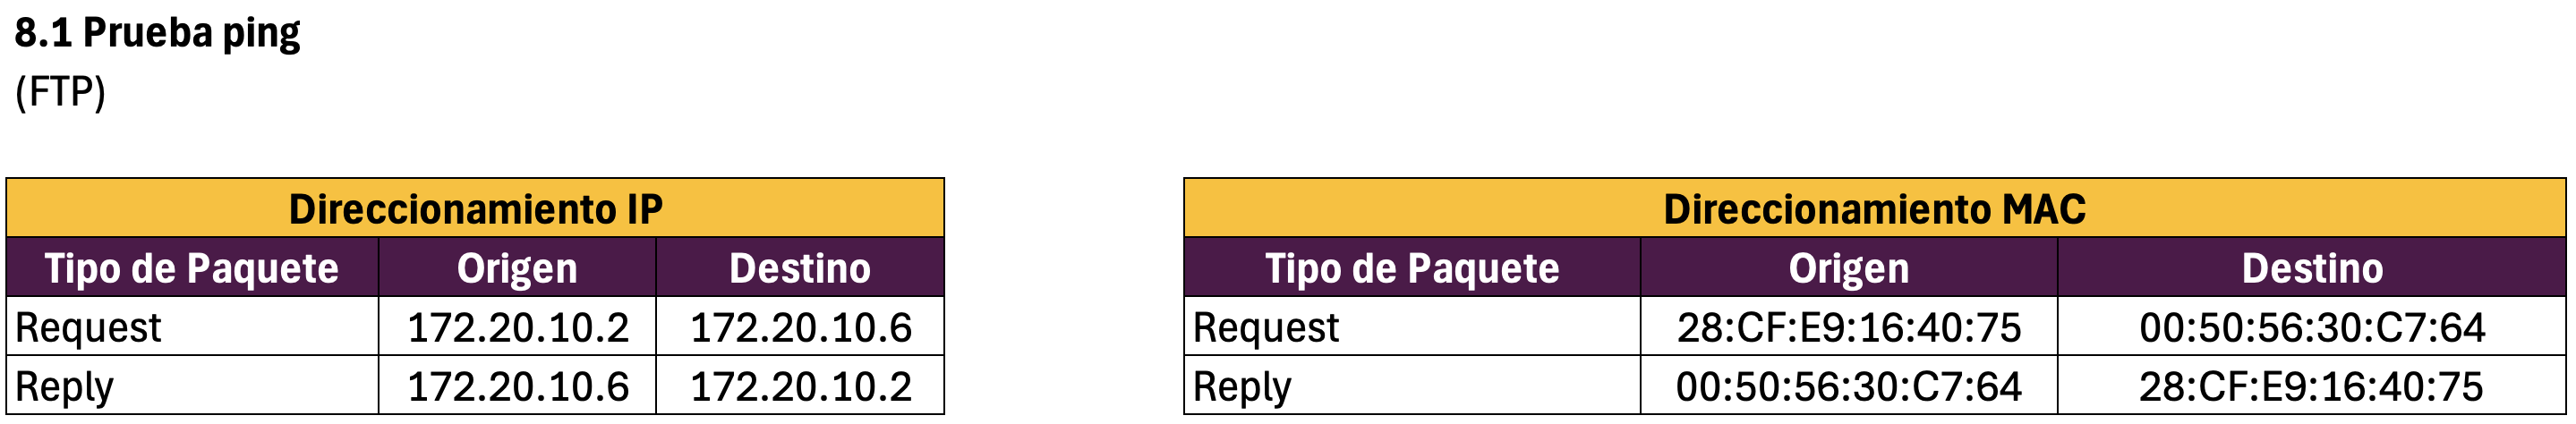
\includegraphics[width=0.85\textwidth]{lab-02-screenshots/8.1-FTP-ping-table}
    \caption{Tabla de IPs y MACs origen/destino}
\end{figure}

\begin{figure}[H]
    \centering
    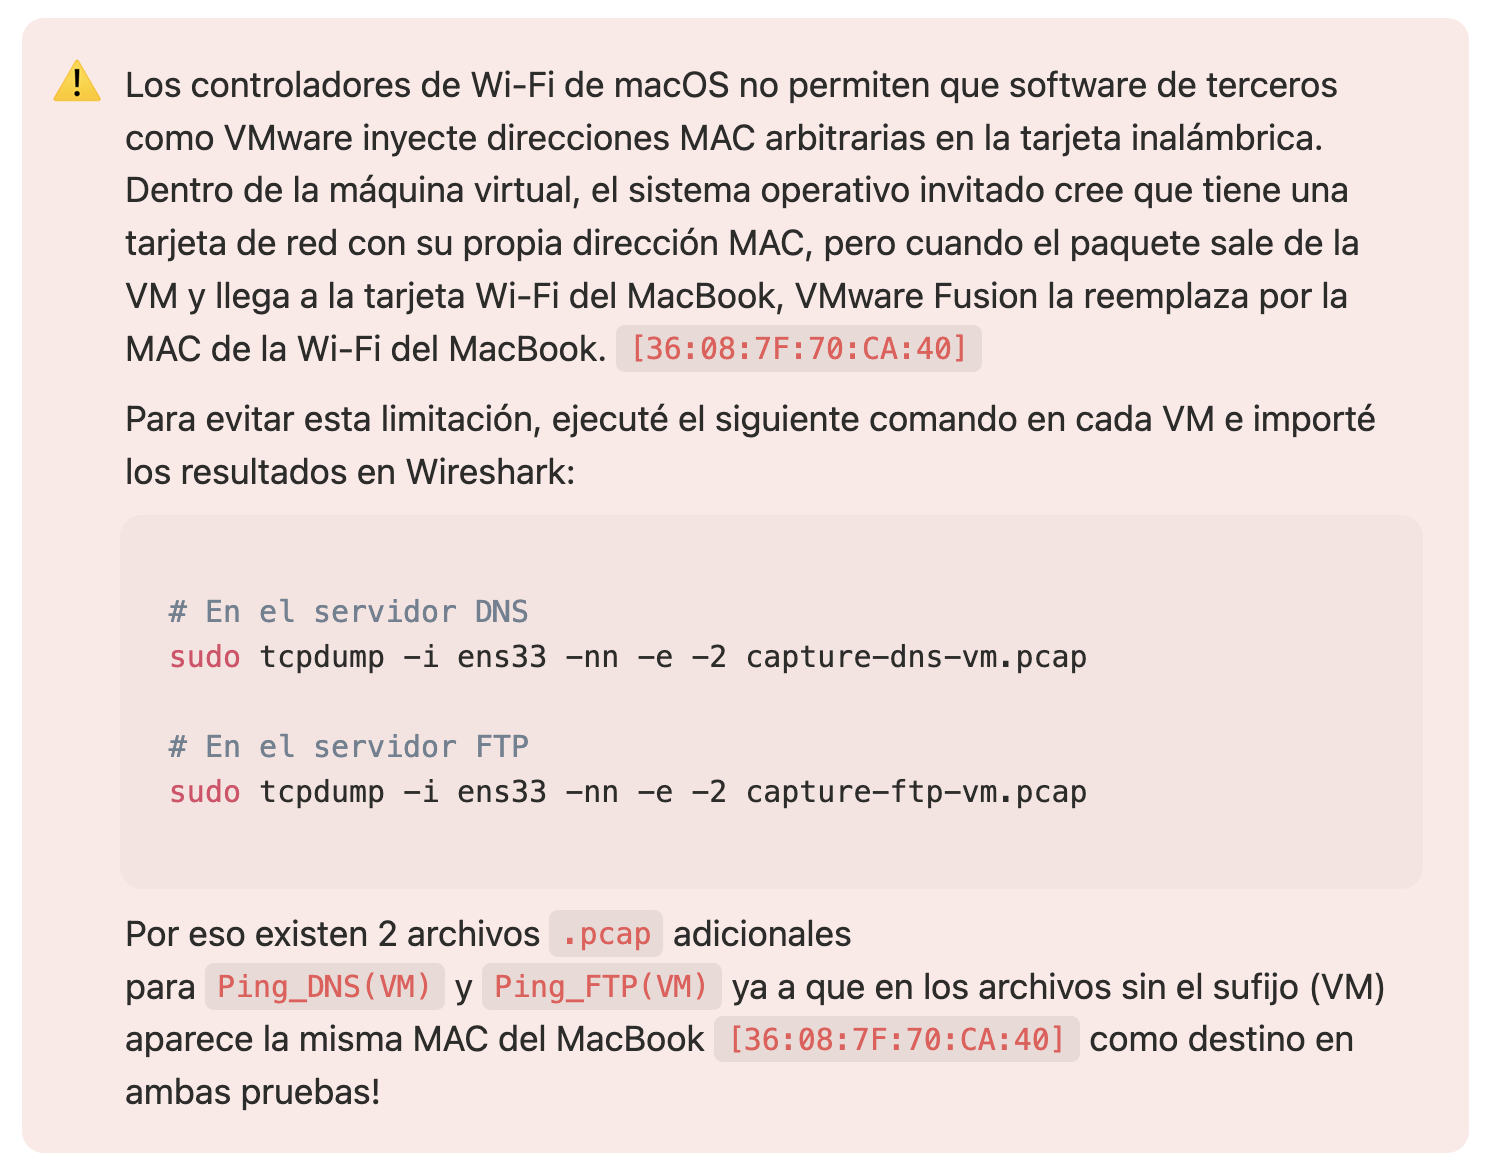
\includegraphics[width=0.85\textwidth]{lab-02-screenshots/8.1-disclaimer}
\end{figure}

%==============================================================
%=====================   8.2   ================================
%==============================================================
\renewcommand{\thesection}{8.\arabic{section}}
\section{Análisis de tráfico del Servicio DNS}

En esta sección se analiza el servicio DNS, que traduce nombres de dominio en direcciones IP para facilitar la comunicación en la red. Se genera y captura tráfico con Wireshark, identificando consultas y respuestas, así como el protocolo de transporte y los puertos utilizados al acceder a un servidor web por IP y por nombre de dominio.


Cuando un cliente necesita comunicarse con un dominio, primero envía al servidor DNS una consulta de tipo \textit{A} para obtener su dirección IPv4 y, en paralelo, una consulta de tipo \textit{AAAA} para la dirección IPv6. El servidor responde con los registros correspondientes, que el cliente almacena en caché. Con la IP resuelta, el cliente ya puede establecer la comunicación (ej. enviar un ping) directamente al servidor destino.  

\subsection{Prueba de conectividad al Servidor Web (IP)}
Cuando se accedió al servidor escribiendo directamente su dirección IP en el ping request, la conexión se estableció de inmediato ya que no fue necesario consultar al DNS y en la captura se observó únicamente tráfico ICMP entre cliente y servidor. El tráfico generado se capturó y se guardó en el archivo \textcolor{blue}{\texttt{Ping\_WEB\_IP.pcap}} El archivo fue analizado en Wireshark con el filtro icmp.

\begin{figure}[H]
    \centering
    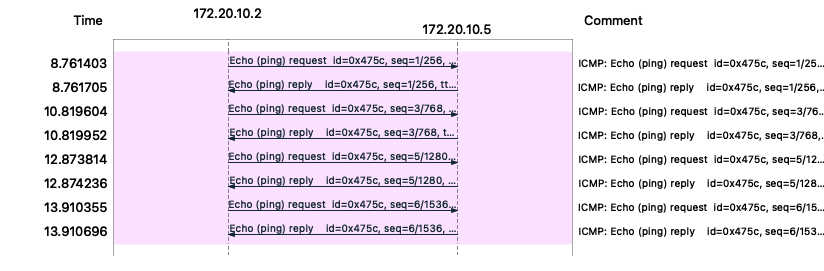
\includegraphics[width=0.85\textwidth]{lab-02-screenshots/8.2-WEB-IP-flow}
    \caption{Flujo de packets en WEB IP ping}
\end{figure}


\begin{figure}[H]
    \centering
    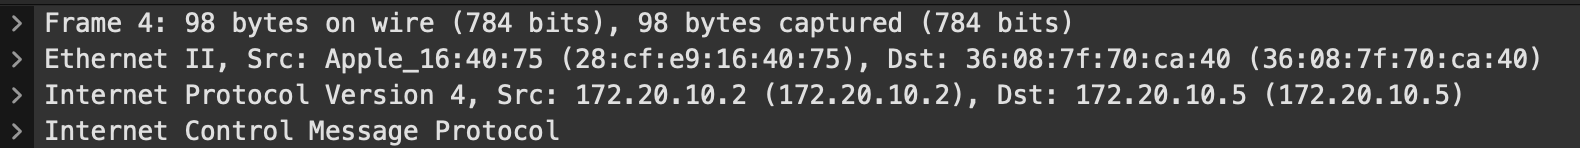
\includegraphics[width=0.85\textwidth]{lab-02-screenshots/8.2-WEB-IP-data}
    \caption{Evidencia de IPs, MACs, y puertos origen/destino}
\end{figure}

\textbf{En esta prueba, no hay resolución DNS.}

\subsection{Prueba de conectividad al Servidor Web (URL)}
Cuando se accedió al servidor utilizando su nombre de dominio en la solicitud de *ping*, el cliente primero realizó consultas de tipo A y AAAA al servidor DNS para obtener la dirección IP correspondiente. Una vez resuelta, se estableció la comunicación con el servidor y en la captura se observó inicialmente el tráfico DNS seguido por el intercambio ICMP entre cliente y servidor. El tráfico generado se capturó y se guardó en el archivo \textcolor{blue}{\texttt{Ping\_WEB.pcap}}, el cual fue analizado en Wireshark aplicando filtros para DNS e ICMP.


\begin{figure}[H]
    \centering
    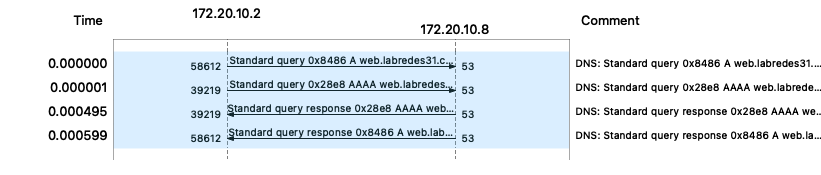
\includegraphics[width=0.85\textwidth]{lab-02-screenshots/8.2-WEB-flow}
    \caption{Flujo de packets en WEB Domain ping}
\end{figure}


\begin{figure}[H]
    \centering
    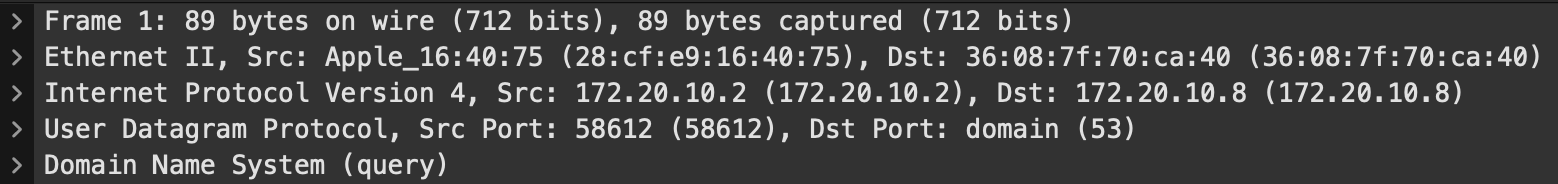
\includegraphics[width=0.85\textwidth]{lab-02-screenshots/8.2-WEB-data}
    \caption{Evidencia de IPs, MACs, y puertos origen/destino}
\end{figure}


\begin{figure}[H]
    \centering
    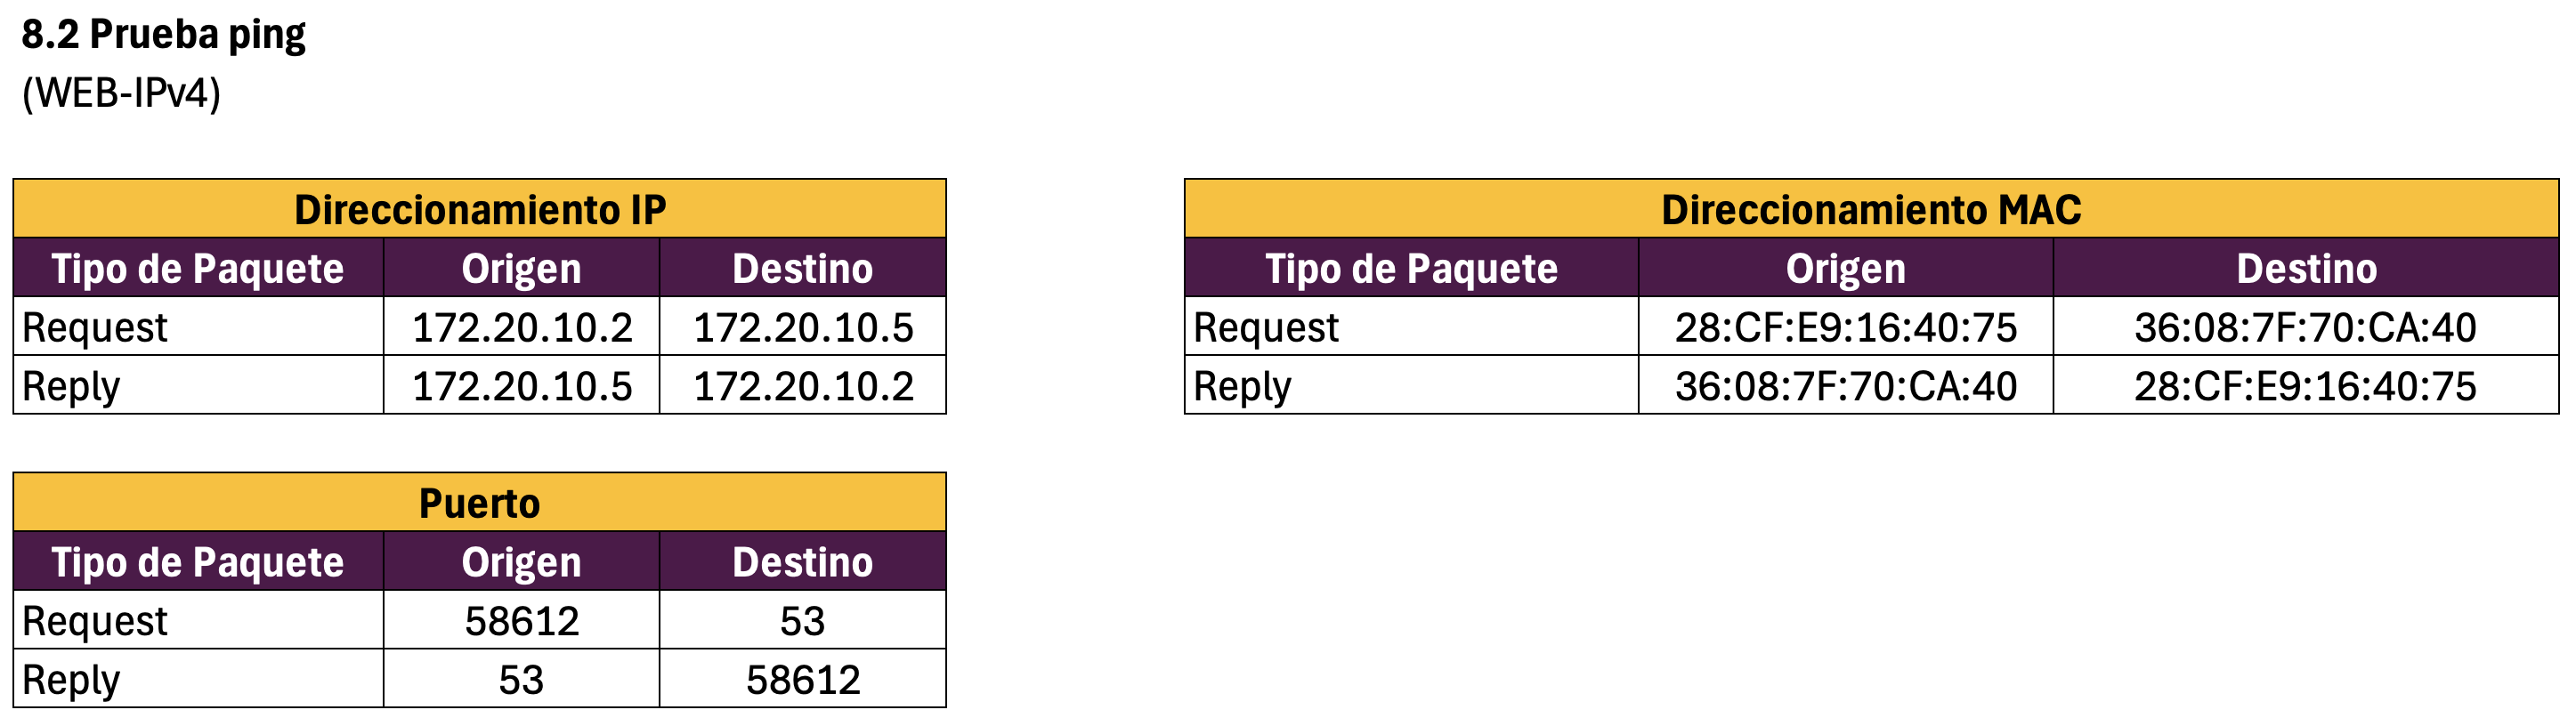
\includegraphics[width=0.85\textwidth]{lab-02-screenshots/8.2-WEB-IP-table}
    \caption{Tabla de IPs, MACs, y puertos origen/destino}
\end{figure}

%==============================================================
%=====================   8.3   ================================
%==============================================================
\renewcommand{\thesection}{8.\arabic{section}}
\section{Análisis de tráfico del Servicio FTP}
\subsection{Conexión al servidor FTP}
\subsection{Descarga de archivo (Download)}
\subsection{Carga de archivo (Upload)}

%==============================================================
%=====================   8.4   ================================
%==============================================================
\renewcommand{\thesection}{8.\arabic{section}}
\section{Análisis de tráfico del Servicio Web}
\subsection{Acceso al servidor web mediante HTTP}

%==============================================================
%=====================   8.5   ================================
%==============================================================
\renewcommand{\thesection}{8.\arabic{section}}
\section{Análisis del protocolo HTTPS realizando navegación en el sitio de YouTube}
\subsection{Navegación en YouTube}
\subsection{Navegación en otros sitios HTTPS}
\subsubsection{https://www.elespectador.com}
\subsubsection{https://www.eltiempo.com}
\subsubsection{https://www.uniandes.edu.co}
\subsubsection{https://www.bancolombia.com}


%==============================================================
%=====================   8.6  ================================
%==============================================================
\renewcommand{\thesection}{8.\arabic{section}}
\section{Análisis del protocolo VoIP}
\subsection{Establecimiento de la llamada}


%==============================================================
%=====================   8.7   ================================
%==============================================================
\renewcommand{\thesection}{8.\arabic{section}}
\section{Análisis del protocolo RTMP}
\subsection{Inicio de la transmisión}


%==============================================================
%=====================   8.7   ================================
%==============================================================
\renewcommand{\thesection}{9.\arabic{section}}
\setcounter{section}{0}
\section{Topología}












\begin{thebibliography}{9}


  \bibitem{kurose_ross}
  Computer Networking, a top-down approach. James Kurose, Keith Ross. Addison-Wesley, 6th ed.

  \end{thebibliography}


\end{document}